\documentclass[12pt, titlepage]{article}

\usepackage{longtable}
\usepackage{fullpage}
\usepackage[round]{natbib}
\usepackage{multirow}
\usepackage{booktabs}
\usepackage{tabularx}
\usepackage{graphicx}
\usepackage{float}
\usepackage{hyperref}
\hypersetup{
    colorlinks,
    citecolor=blue,
    filecolor=black,
    linkcolor=red,
    urlcolor=blue
}

\usepackage{xr}
\externaldocument[SRS-]{../../SRS-IEEE/SRS}

\newcommand{\rref}[1]{FR\ref{SRS-#1}}
\newcommand{\nfrref}[1]{NFR\ref{SRS-#1}}
\newcommand{\prref}[1]{PR\ref{SRS-#1}}

\input{../../Comments.text}
\input{../../Common.text}

\newcounter{acnum}
\newcommand{\actheacnum}{AC\theacnum}
\newcommand{\acref}[1]{AC\ref{#1}}

\newcounter{ucnum}
\newcommand{\uctheucnum}{UC\theucnum}
\newcommand{\uref}[1]{UC\ref{#1}}

\newcounter{mnum}
\newcommand{\mthemnum}{M\themnum}
\newcommand{\mref}[1]{M\ref{#1}}

\begin{document}

\title{Module Guide for \progname{}} 
\author{\authname}
\date{\today}

\maketitle

\pagenumbering{roman}

\section{Revision History}

\begin{tabularx}{\textwidth}{p{3cm}p{2cm}X}
\toprule {\bf Date} & {\bf Version} & {\bf Notes}\\
\midrule
2026-11-11 & 0.1 & Initial draft of the anticipated and unlikely changes, the module hierarchy, and the module secrets\\
2026-11-15 & 0.2 & Added the requirements-to-modules traceability table, with references to the SRS\\
2026-11-17 & 0.3 & Revised the module decomposition and secrets; added the uses hierarchy, the anticipated-changes traceability table, module services, and the Online Daily Challenge Manager module\\
2026-11-18 & 1.0 & Completed the traceability between the requirements (functional, non-functional, and privacy and data retention) and the modules, and added the Generative AI Use Disclosure (Rev $-1$ submission)\\
\bottomrule
\end{tabularx}

\newpage

\section{Reference Material}

This section records information for easy reference. 

\subsection{Abbreviations and Acronyms}

\renewcommand{\arraystretch}{1.2}
\begin{tabular}{l l} 
  \toprule		
  \textbf{symbol} & \textbf{description}\\
  \midrule 
  AC & Anticipated Change\\
  DAG & Directed Acyclic Graph \\
  M & Module \\
  MG & Module Guide \\
  OS & Operating System \\
  R & Requirement\\
  SC & Scientific Computing \\
  SRS & Software Requirements Specification\\
  \progname & Explanation of program name\\
  UC & Unlikely Change \\
  \wss{etc.} & \wss{...}\\
  \bottomrule
\end{tabular}\\

\newpage

\tableofcontents

\listoftables

\listoffigures

\newpage

\pagenumbering{arabic}

\section{Introduction}

Decomposing a system into modules is a commonly accepted approach to developing
software.  A module is a work assignment for a programmer or programming
team~\citep{ParnasEtAl1984}.  We advocate a decomposition
based on the principle of information hiding~\citep{Parnas1972a}.  This
principle supports design for change, because the ``secrets'' that each module
hides represent likely future changes.  Design for change is valuable in SC,
where modifications are frequent, especially during initial development as the
solution space is explored.  

Our design follows the rules layed out by \citet{ParnasEtAl1984}, as follows:
\begin{itemize}
\item System details that are likely to change independently should be the
  secrets of separate modules.
\item Each data structure is implemented in only one module.
\item Any other program that requires information stored in a module's data
  structures must obtain it by calling access programs belonging to that module.
\end{itemize}

After completing the first stage of the design, the Software Requirements
Specification (SRS), the Module Guide (MG) is developed~\citep{ParnasEtAl1984}. The MG
specifies the modular structure of the system and is intended to allow both
designers and maintainers to easily identify the parts of the software.  The
potential readers of this document are as follows:

\begin{itemize}
\item New project members: This document can be a guide for a new project member
  to easily understand the overall structure and quickly find the
  relevant modules they are searching for.
\item Maintainers: The hierarchical structure of the module guide improves the
  maintainers' understanding when they need to make changes to the system. It is
  important for a maintainer to update the relevant sections of the document
  after changes have been made.
\item Designers: Once the module guide has been written, it can be used to
  check for consistency, feasibility, and flexibility. Designers can verify the
  system in various ways, such as consistency among modules, feasibility of the
  decomposition, and flexibility of the design.
\end{itemize}

The rest of the document is organized as follows. Section
\ref{SecChange} lists the anticipated and unlikely changes of the software
requirements. Section \ref{SecMH} summarizes the module decomposition that
was constructed according to the likely changes. Section \ref{SecConnection}
specifies the connections between the software requirements and the
modules. Section \ref{SecMD} gives a detailed description of the
modules. Section \ref{SecTM} includes two traceability matrices. One checks
the completeness of the design against the requirements provided in the SRS. The
other shows the relation between anticipated changes and the modules. Section
\ref{SecUse} describes the use relation between modules.

\section{Anticipated and Unlikely Changes} \label{SecChange}

This section lists possible changes to the system. According to the likeliness
of the change, the possible changes are classified into two
categories. Anticipated changes are listed in Section \ref{SecAchange}, and
unlikely changes are listed in Section \ref{SecUchange}.

\subsection{Anticipated Changes} \label{SecAchange}

Anticipated changes are the source of the information that is to be hidden
inside the modules. Ideally, changing one of the anticipated changes will only
require changing the one module that hides the associated decision. The approach
adapted here is called design for
change.

\begin{description}
\item [\refstepcounter{acnum} \actheacnum \label{acHardware}:] The specific hardware and browser environment on which the software is running.
\item [\refstepcounter{acnum} \actheacnum \label{acUI}:] How user input is received and translated into commands, and how the application state is presented to the user.
\item [\refstepcounter{acnum} \actheacnum \label{acCR}:] The data structure used to store the numbers of the magic cube and look them up by cell.
\item [\refstepcounter{acnum} \actheacnum \label{acN}:] The screens and menus in the application and the transitions/structure between them.
\item [\refstepcounter{acnum} \actheacnum \label{acRC}:] The sequence of steps within a round and within each task.
\item [\refstepcounter{acnum} \actheacnum \label{acR}:] The rules of a round including the number and sequence of tasks, the cube order, and the valid line types for the tasks.
\item [\refstepcounter{acnum} \actheacnum \label{acRG}:] The algorithms and techniques used to generate a gameplay round given the rules of a round.
\item [\refstepcounter{acnum} \actheacnum \label{acS}:] The scoring system (i.e., how score is calculated for a task and round).
\item [\refstepcounter{acnum} \actheacnum \label{acTG}:] The algorithms used to compute the cells of a line from a starter and a line type.
\item [\refstepcounter{acnum} \actheacnum \label{acUD}:] How user data is saved.
\item [\refstepcounter{acnum} \actheacnum \label{acGD}:] How and when game state data is saved.
\item [\refstepcounter{acnum} \actheacnum \label{acRE}:] The algorithms and techniques used to render the 3D space and game state.
\item [\refstepcounter{acnum} \actheacnum \label{acAA}:] How user accounts are authenticated and managed.
\item [\refstepcounter{acnum} \actheacnum \label{acL}:] The structure and types of leaderboards presented.
\item [\refstepcounter{acnum} \actheacnum \label{acDC}:] How the daily challenge is obtained and played on the user's device.
\item [\refstepcounter{acnum} \actheacnum \label{acT}:] The content and state flow of the tutorial.
\item [\refstepcounter{acnum} \actheacnum \label{acSE}:] The application settings available.
\item [\refstepcounter{acnum} \actheacnum \label{acNB}:] The number base in which values are shown to and entered by the user.
\item [\refstepcounter{acnum} \actheacnum \label{acSCM}:] How the application communicates with the online server (e.g., the server provider, its interface, and the network protocol).
\item [\refstepcounter{acnum} \actheacnum \label{acDCM}:] How the daily round is created, scheduled, and stored on the online server so that every user receives the same round.
\end{description}

These anticipated changes include the likely changes listed in the SRS: LC2
(the contrast standard) is covered by \acref{acUI}; LC3 (additional number
bases and cube orders) by \acref{acR} and \acref{acNB}; LC4 (new game modes and
rulesets) by \acref{acR} and \acref{acRG}; LC5 (the scoring mechanism) by
\acref{acS}; LC6 (how often the game is saved) by \acref{acGD}; LC7 (the 3D
visualization) by \acref{acRE}; and LC8 (the daily challenge) by \acref{acDC} and \acref{acDCM}.
LC1 (the 100\,ms response targets) has no corresponding anticipated change,
because it changes a performance target that the design must meet rather than
a design decision hidden by a module.

\wss{Anticipated changes relate to changes that would be made in requirements,
design or implementation choices.  They are not related to changes that are made
at run-time, like the values of parameters.}

\subsection{Unlikely Changes} \label{SecUchange}

The module design should be as general as possible. However, a general system is
more complex. Sometimes this complexity is not necessary. Fixing some design
decisions at the system architecture stage can simplify the software design. If
these decision should later need to be changed, then many parts of the design
will potentially need to be modified. Hence, it is not intended that these
decisions will be changed.

\begin{description}
\item [\refstepcounter{ucnum} \uctheucnum \label{ucI}:] The game control input devices (keyboard/mouse or touchscreen).
\item [\refstepcounter{ucnum} \uctheucnum \label{ucO}:] The game output devices (screen).
\item [\refstepcounter{ucnum} \uctheucnum \label{ucWB}:] The game is web-browser based.
\item [\refstepcounter{ucnum} \uctheucnum \label{ucM}:] The mathematical properties of magic cubes upon which the game logic is based.
\item [\refstepcounter{ucnum} \uctheucnum \label{ucD}:] Gameplay logic operates on decimal-base values, independent of the number base shown to the user.
\end{description}

\section{Module Hierarchy} \label{SecMH}

This section provides an overview of the module design. Modules are summarized
in a hierarchy decomposed by secrets in Table \ref{TblMH}. The modules listed
below, which are leaves in the hierarchy tree, are the modules that will
actually be implemented.

\begin{description}
\item [\refstepcounter{mnum} \mthemnum \label{mVH}:] Virtual Hardware Module

\item [\refstepcounter{mnum} \mthemnum \label{mUI}:] User Interface Module
\item [\refstepcounter{mnum} \mthemnum \label{mRE}:] Rendering Module
\item [\refstepcounter{mnum} \mthemnum \label{mN}:] Navigation Module
\item [\refstepcounter{mnum} \mthemnum \label{mRC}:] Round Control Module
\item [\refstepcounter{mnum} \mthemnum \label{mR}:] Ruleset Module
\item [\refstepcounter{mnum} \mthemnum \label{mSC}:] Scoring Module
\item [\refstepcounter{mnum} \mthemnum \label{mUM}:] User Management Module
\item [\refstepcounter{mnum} \mthemnum \label{mL}:] Leaderboard Module
\item [\refstepcounter{mnum} \mthemnum \label{mDC}:] Daily Challenge Module
\item [\refstepcounter{mnum} \mthemnum \label{mT}:] Tutorial Module
\item [\refstepcounter{mnum} \mthemnum \label{mSE}:] Settings Module

\item [\refstepcounter{mnum} \mthemnum \label{mCR}:] Cube Representation Module
\item [\refstepcounter{mnum} \mthemnum \label{mGDM}:] Game Data Management Module
\item [\refstepcounter{mnum} \mthemnum \label{mRG}:] Round Generation Module
\item [\refstepcounter{mnum} \mthemnum \label{mTG}:] Line Geometry Module
\item [\refstepcounter{mnum} \mthemnum \label{mUDM}:] User Data Management Module
\item [\refstepcounter{mnum} \mthemnum \label{mNBT}:] Number Base Translation Module
\item [\refstepcounter{mnum} \mthemnum \label{mSCM}:] Server Communication Module
\item [\refstepcounter{mnum} \mthemnum \label{mDCM}:] Online Daily Challenge Manager Module
\end{description}


\begin{table}[h!]
\centering
\begin{tabular}{p{0.3\textwidth} p{0.6\textwidth}}
\toprule
\textbf{Level 1} & \textbf{Level 2}\\
\midrule

Hardware-Hiding Module
& Virtual Hardware Module\\
\midrule

\multirow{11}{0.3\textwidth}{Behaviour-Hiding Module}
& User Interface Module\\
& Rendering Module\\
& Navigation Module\\
& Round Control Module\\
& Ruleset Module\\
& Scoring Module\\
& User Management Module\\
& Leaderboard Module\\
& Daily Challenge Module\\
& Tutorial Module\\
& Settings Module\\
\midrule

\multirow{8}{0.3\textwidth}{Software Decision Module}
& Cube Representation Module\\
& Game Data Management Module\\
& Round Generation Module\\
& Line Geometry Module\\
& User Data Management Module\\
& Number Base Translation Module\\
& Server Communication Module\\
& Online Daily Challenge Manager Module\\
\bottomrule

\end{tabular}
\caption{Module Hierarchy}
\label{TblMH}
\end{table}

\section{Connection Between Requirements and Design} \label{SecConnection}

The design of the system is intended to satisfy the requirements developed in
the SRS. In this stage, the system is decomposed into modules. The connection
between requirements and modules is listed in Table~\ref{TblRT}.

\wss{The intention of this section is to document decisions that are made
  ``between'' the requirements and the design.  To satisfy some requirements,
  design decisions need to be made.  Rather than make these decisions implicit,
  they are explicitly recorded here.  For instance, if a program has security
  requirements, a specific design decision may be made to satisfy those
  requirements with a password.}

\section{Module Decomposition} \label{SecMD}

Modules are decomposed according to the principle of ``information hiding''
proposed by \citet{ParnasEtAl1984}. The \emph{Secrets} field in a module
decomposition is a brief statement of the design decision hidden by the
module. The \emph{Services} field specifies \emph{what} the module will do
without documenting \emph{how} to do it. For each module, a suggestion for the
implementing software is given under the \emph{Implemented By} title. If the
entry is \emph{OS}, this means that the module is provided by the operating
system or by standard programming language libraries.  \emph{\progname{}} means the
module will be implemented by the \progname{} software.

Only the leaf modules in the hierarchy have to be implemented. If a dash
(\emph{--}) is shown, this means that the module is not a leaf and will not have
to be implemented.

Each module hides one secret, with two deliberate exceptions. \mref{mUI}
hides both the mapping from input to commands and the presentation of the
application state, because both depend on the same device library and screen
layout and are expected to change together. \mref{mUM} hides both the
management of accounts and the computation of personal statistics, because
statistics exist only for an account and are computed from the same recorded
data that the account owns.

\subsection{Hardware Hiding Modules}

\begin{description}
\item[Secrets:]The data structure and algorithm used to implement the virtual
  hardware.
\item[Services:]Serves as a virtual hardware used by the rest of the
  system. This module provides the interface between the hardware and the
  software. So, the system can use it to display outputs or to accept inputs.
\item[Implemented By:] --
\end{description}

\subsubsection{Virtual Hardware Module (\mref{mVH})}

\begin{description}
\item[Secrets:] The interface to the input and output devices.
\item[Services:]
\item[Implemented By:] pygame-ce, pygbag, and the web browser
\item[Type of Module:]
\end{description}

\subsection{Behaviour-Hiding Module}

\begin{description}
\item[Secrets:]The contents of the required behaviours.
\item[Services:]Includes programs that provide externally visible behaviour of
  the system as specified in the software requirements specification (SRS)
  documents. This module serves as a communication layer between the
  hardware-hiding module and the software decision module. The programs in this
  module will need to change if there are changes in the SRS.
\item[Implemented By:] --
\end{description}

\subsubsection{User Interface Module (\mref{mUI})}

\begin{description}
\item[Secrets:] The mapping from user input to commands, and the presentation of the application state to the user, including the drawing of every screen.
\item[Services:] Reads device input and converts it into commands for \mref{mN}, converting typed answers from the display base with \mref{mNBT}. Draws each screen from the content provided by \mref{mN} and, for the game space, from the view produced by \mref{mRE}.
\item[Implemented By:]
\item[Type of Module:]
\end{description}

\subsubsection{Rendering Module (\mref{mRE})}

\begin{description}
\item[Secrets:] The algorithms to translate the 3D space and game state into a 2D view, including layer isolation and highlighting.
\item[Services:] Produces the 2D view of the game space from the round state read from \mref{mRC}, for \mref{mUI} to display. It does not display the view itself.
\item[Implemented By:]
\item[Type of Module:]
\end{description}

\subsubsection{Navigation Module (\mref{mN})}

\begin{description}
\item[Secrets:] The structure of the application's screens and menus (including the settings screen) and the transitions between them, including those into and out of a game round.
\item[Services:] Tracks the current screen, carries out the commands passed in from \mref{mUI}, and provides the content of the current screen to \mref{mUI}.
\item[Implemented By:]
\item[Type of Module:]
\end{description}

\subsubsection{Round Control Module (\mref{mRC})}

\begin{description}
\item[Secrets:] The state and progression of a round and the tasks within it (e.g., the selected cell and the player's answers).
\item[Services:] Plays a round given its plane, orientation, starter, and line types; carries out the player's actions and checks them against the ruleset; provides snapshots to \mref{mGDM} for autosave and resume; and records the result through \mref{mUDM} unless the round is marked as a tutorial round. Its read-only access programs provide the round state to \mref{mRE}.
\item[Implemented By:]
\item[Type of Module:]
\end{description}

\subsubsection{Ruleset Module (\mref{mR})}

\begin{description}
\item[Secrets:] The rules of a gameplay round including the number and sequence of tasks, cube order, number-base, additional number counts for each task, valid line-types (e.g., complement, diagonal), and which scoring scheme applies.
\item[Services:]
\item[Implemented By:]
\item[Type of Module:]
\end{description}

\subsubsection{Scoring Module (\mref{mSC})}

\begin{description}
\item[Secrets:] The available scoring schemes, and the algorithms each uses to calculate task/round scores and performance metrics.
\item[Services:]
\item[Implemented By:]
\item[Type of Module:]
\end{description}

\subsubsection{User Management Module (\mref{mUM})}

\begin{description}
\item[Secrets:] The algorithms used to authenticate users and manage user accounts (e.g., create/delete account, login/logout, password reset), to keep track of the current user's session (logged in or playing as a guest), and to compute a user's personal statistics (e.g., completed rounds, highest and average score, fastest round time) from their recorded round results.
\item[Services:] Carries out account actions, and on login or logout sets the current user (or guest) in \mref{mUDM}. Computes personal statistics from the results read from \mref{mUDM} when they are viewed.
\item[Implemented By:]
\item[Type of Module:]
\end{description}

\subsubsection{Leaderboard Module (\mref{mL})}

\begin{description}
\item[Secrets:] The data structure and algorithms used to select and rank recorded round results into leaderboards (e.g., by scoring base, score or time, all-time or daily challenge).
\item[Services:]
\item[Implemented By:]
\item[Type of Module:]
\end{description}

\subsubsection{Daily Challenge Module (\mref{mDC})}

\begin{description}
\item[Secrets:] How the day's round is obtained from the online server and played on the user's device.
\item[Services:] Fetches the day's round from \mref{mDCM} through \mref{mSCM} and plays it through \mref{mRC}, marked as a daily challenge round so its result is recorded for that day's leaderboard.
\item[Implemented By:]
\item[Type of Module:]
\end{description}

\subsubsection{Tutorial Module (\mref{mT})}

\begin{description}
\item[Secrets:] The content and order of the tutorial's steps, and the fixed round they are played on.
\item[Services:] Plays the fixed round through \mref{mRC}, marked as a tutorial round so its result is not recorded, and provides the instruction for the step the player has reached.
\item[Implemented By:]
\item[Type of Module:]
\end{description}

\subsubsection{Settings Module (\mref{mSE})}

\begin{description}
\item[Secrets:] The application's settings and the algorithms to access and modify them (e.g., turning off animations and configuring the play-time reminder).
\item[Services:]
\item[Implemented By:]
\item[Type of Module:]
\end{description}

\subsection{Software Decision Module}

\begin{description}
\item[Secrets:] The design decision based on mathematical theorems, physical
  facts, or programming considerations. The secrets of this module are
  \emph{not} described in the SRS.
\item[Services:] Includes data structure and algorithms used in the system that
  do not provide direct interaction with the user. 
  % Changes in these modules are more likely to be motivated by a desire to
  % improve performance than by externally imposed changes.
\item[Implemented By:] --
\end{description}

\subsubsection{Cube Representation Module (\mref{mCR})}

\begin{description}
\item[Secrets:] The data structure used to store the numbers of the magic cube and look them up by cell.
\item[Services:] Builds a cube of a given size from its numbers, checks that each number appears exactly once, and returns the number in a given cell. The cube size is passed in by the caller, so this module does not use \mref{mR}.
\item[Implemented By:]
\item[Type of Module:]
\end{description}

\subsubsection{Game Data Management Module (\mref{mGDM})}

\begin{description}
\item[Secrets:] The algorithms to save, modify, delete, and load snapshots of the in-progress round, stored on the device for autosave and resume.
\item[Services:]
\item[Implemented By:]
\item[Type of Module:]
\end{description}

\subsubsection{Round Generation Module (\mref{mRG})}

\begin{description}
\item[Secrets:] The algorithms used to choose a round's plane, orientation, starter, and the line type for each task, consistent with the ruleset.
\item[Services:]
\item[Implemented By:]
\item[Type of Module:]
\end{description}

\subsubsection{Line Geometry Module (\mref{mTG})}

\begin{description}
\item[Secrets:] The algorithms used to compute the cells of a line in the cube from a starter and a line type, including wrapping for split lines, whether a line is continuous, and the order in which the line is traced.
\item[Services:] Given a cube size, a starter cell, and a line type, returns the line's other cells in the order they are traced, and whether the line is continuous or split. The cube size is passed in by the caller, so this module does not use \mref{mR}.
\item[Implemented By:]
\item[Type of Module:]
\end{description}

\subsubsection{User Data Management Module (\mref{mUDM})}

\begin{description}
\item[Secrets:] The data structure and algorithms to save, modify, delete, and load user data, including account records, settings, used starters, and recorded round results (the source of personal statistics and leaderboard rankings).
\item[Services:] Saves and loads data for the current user set by \mref{mUM}. A guest's data is kept only on the device; a logged-in user's data is kept on the server through \mref{mSCM}. Also loads the recorded round results of all users from the server, for \mref{mL} to rank.
\item[Implemented By:]
\item[Type of Module:]
\end{description}

\subsubsection{Number Base Translation Module (\mref{mNBT})}

\begin{description}
\item[Secrets:] The algorithms to convert between the decimal-base values used in gameplay logic and their external user representation in the given number base.
\item[Services:]
\item[Implemented By:]
\item[Type of Module:]
\end{description}

\subsubsection{Server Communication Module (\mref{mSCM})}

\begin{description}
\item[Secrets:] The protocol and interface used to exchange data with the online server, including the server's request formats, secure transport, and the handling of failed requests.
\item[Services:]
\item[Implemented By:]
\item[Type of Module:]
\end{description}

\subsubsection{Online Daily Challenge Manager Module (\mref{mDCM})}

\begin{description}
\item[Secrets:] The algorithms used to create, schedule, and store the daily round on the online server so that every user receives the same round.
\item[Services:] Creates one round each day using \mref{mRG} and the daily challenge ruleset from \mref{mR}, and serves that round to every client that requests it. Runs on the online server, not on the user's device.
\item[Implemented By:]
\item[Type of Module:]
\end{description}

\section{Traceability Matrix} \label{SecTM}

This section shows two traceability matrices: between the modules and the
requirements and between the modules and the anticipated changes.

% the table should use mref, the requirements should be named, use something
% like fref
\begin{longtable}{p{0.3\textwidth} p{0.6\textwidth}}
\caption{Trace Between Requirements and Modules} \label{TblRT}\\
\toprule
\textbf{Req.} & \textbf{Modules}\\
\midrule
\endfirsthead
\toprule
\textbf{Req.} & \textbf{Modules}\\
\midrule
\endhead
\bottomrule
\endlastfoot
\rref{FR_StartRound} & \mref{ADD REF}\\
\rref{FR_SelectPlane} & \\
\rref{FR_SelectOrientation} & \\
\rref{FR_ChooseBase} & \\
\rref{FR_ShowStarter} & \\
\rref{FR_NoRepeatStarter} & \\
\rref{FR_TaskOrder} & \\
\rref{FR_CellFeedback} & \\
\rref{FR_Task1} & \\
\rref{FR_Task2} & \\
\rref{FR_Task3} & \\
\rref{FR_Task4} & \\
\rref{FR_Task5} & \\
\rref{FR_Task6} & \\
\rref{FR_Task7} & \\
\rref{FR_Task8} & \\
\rref{FR_ChooseExtra} & \\
\rref{FR_AdditionColumn} & \\
\rref{FR_AdditionCheck} & \\
\rref{FR_SubtractionPrompt} & \\
\rref{FR_SubtractionCheck} & \\
\rref{FR_InputValidation} & \\
\rref{FR_UnrecognizedInput} & \\
\rref{FR_NextTask} & \\
\rref{FR_EndRound} & \\
\rref{FR_VerifyTask} & \\
\rref{FR_BasicPoints} & \\
\rref{FR_TimedScore} & \\
\rref{FR_Totals} & \\
\rref{FR_StopGame} & \\
\rref{FR_Autosave} & \\
\rref{FR_Resume} & \\
\rref{FR_3DView} & \\
\rref{FR_3DNavigate} & \\
\rref{FR_3DLayers} & \\
\rref{FR_3DHighlight} & \\
\rref{FR_PerformanceWarning} & \\
\rref{FR_Tutorial} & \\
\rref{FR_ExplainCell} & \\
\rref{FR_Hint} & \\
\rref{FR_SolutionPath} & \\
\rref{FR_GuestPlay} & \\
\rref{FR_CreateAccount} & \\
\rref{FR_UsernameRules} & \\
\rref{FR_Login} & \\
\rref{FR_PasswordReset} & \\
\rref{FR_RecordRound} & \\
\rref{FR_Statistics} & \\
\rref{FR_Leaderboards} & \\
\rref{FR_LeaderboardIntegrity} & \\
\rref{FR_DailyChallenge} & \\
\rref{FR_ShareResults} & \\
\rref{FR_DeleteAccount} & \\
\rref{FR_PlayTimeReminder} & \\
\rref{FR_DisableAnimations} & \\
\midrule
\nfrref{NFR_1} & \mref{mUI}, \mref{mRE}, \mref{mCR}, \mref{mGDM}\\
\nfrref{NFR_2} & \mref{mUI}, \mref{mRE}, \mref{mGDM}\\
\nfrref{NFR_3} & \mref{mUI}, \mref{mRE}\\
\nfrref{NFR_4} & \mref{mUI}, \mref{mRE}\\
\nfrref{NFR_5} & \mref{mUI}, \mref{mRE}\\
\nfrref{NFR_6} & \mref{mUI}, \mref{mRE}\\
\nfrref{NFR_7} & \mref{mUI}, \mref{mRE}, \mref{mGDM}, \mref{mUM}, \mref{mSCM}, \mref{mRC}, \mref{mR}\\
\nfrref{NFR_8} & \mref{mGDM}, \mref{mRC}, \mref{mR}\\
\nfrref{NFR_9} & \mref{mVH}\\
\nfrref{NFR_10} & \mref{mVH}\\
\nfrref{NFR_11} & \mref{mGDM}\\
\nfrref{NFR_12} & \mref{mR}, \mref{mRC}\\
\nfrref{NFR_13} & \mref{mUM}, \mref{mUDM}, \mref{mSCM}, \mref{mDCM}\\
\nfrref{NFR_14} & \mref{mUM}, \mref{mUDM}, \mref{mSCM}\\
\nfrref{NFR_15} & \mref{mUM}, \mref{mUDM}, \mref{mSCM}\\
\nfrref{NFR_16} & \mref{mUDM}, \mref{mGDM}\\
\nfrref{NFR_17} & \mref{mUM}, \mref{mUDM}\\
\nfrref{NFR_18} & \mref{mUI}\\
\nfrref{NFR_19} & \mref{mRE}\\
\midrule
\prref{PR_1} & \mref{ADD REF} \\
\prref{PR_2} & \\
\prref{PR_3} & \\
\prref{PR_4} & \\
\prref{PR_5} & \\
\prref{PR_6} & \\
\prref{PR_7} & \\
\prref{PR_8} & \\
\prref{PR_9} & \\
\prref{PR_10} & \\
\end{longtable}

\begin{table}[H]
\centering
\begin{tabular}{p{0.2\textwidth} p{0.6\textwidth}}
\toprule
\textbf{AC} & \textbf{Modules}\\
\midrule
\acref{acHardware} & \mref{mVH}\\
\acref{acUI} & \mref{mUI}\\
\acref{acCR} & \mref{mCR}\\
\acref{acN} & \mref{mN}\\
\acref{acRC} & \mref{mRC}\\
\acref{acR} & \mref{mR}\\
\acref{acRG} & \mref{mRG}\\
\acref{acS} & \mref{mSC}\\
\acref{acTG} & \mref{mTG}\\
\acref{acUD} & \mref{mUDM}\\
\acref{acGD} & \mref{mGDM}\\
\acref{acRE} & \mref{mRE}\\
\acref{acAA} & \mref{mUM}\\
\acref{acL} & \mref{mL}\\
\acref{acDC} & \mref{mDC}\\
\acref{acT} & \mref{mT}\\
\acref{acSE} & \mref{mSE}\\
\acref{acNB} & \mref{mNBT}\\
\acref{acSCM} & \mref{mSCM}\\
\acref{acDCM} & \mref{mDCM}\\
\bottomrule
\end{tabular}
\caption{Trace Between Anticipated Changes and Modules}
\label{TblACT}
\end{table}

\section{Use Hierarchy Between Modules} \label{SecUse}

In this section, the uses hierarchy between modules is
provided. \citet{Parnas1978} said of two programs A and B that A {\em uses} B if
correct execution of B may be necessary for A to complete the task described in
its specification. That is, A {\em uses} B if there exist situations in which
the correct functioning of A depends upon the availability of a correct
implementation of B.  Figure \ref{FigUH} illustrates the use relation between
the modules. It can be seen that the graph is a directed acyclic graph
(DAG). Each level of the hierarchy offers a testable and usable subset of the
system, and modules in the higher level of the hierarchy are essentially simpler
because they use modules from the lower levels.

An arrow from module A to module B means that A uses B. Only direct uses are
shown; since the relation is transitive, indirect uses follow from the arrows.
Modules \mref{mVH}, \mref{mR}, \mref{mSC}, \mref{mCR}, \mref{mGDM},
\mref{mTG}, \mref{mNBT}, and \mref{mSCM} use no other module. \mref{mUI} sits
at the top because it is the only point of contact with the user: it reads
input through \mref{mVH}, passes the resulting commands to \mref{mN}, and
draws every screen through \mref{mVH}, using data provided by \mref{mN} and,
for the game space, the projected view produced by \mref{mRE}. No other module uses
\mref{mUI}, so all game logic, including \mref{mN}, \mref{mRC}, and \mref{mT},
can be tested without launching the user interface or rendering the cube
(\nfrref{NFR_7}, \nfrref{NFR_8}).

Every Software Decision module is used by at least one other module, except
\mref{mDCM}. It runs on the online server rather than on the user's device, and
\mref{mDC} reaches the round it serves only through \mref{mSCM}, so no module on
the device depends on how the daily round is created. \mref{mSCM} is used only
by \mref{mUDM} and \mref{mDC}, so that no other module depends on how the
application communicates with the online server.

\begin{figure}[H]
\centering
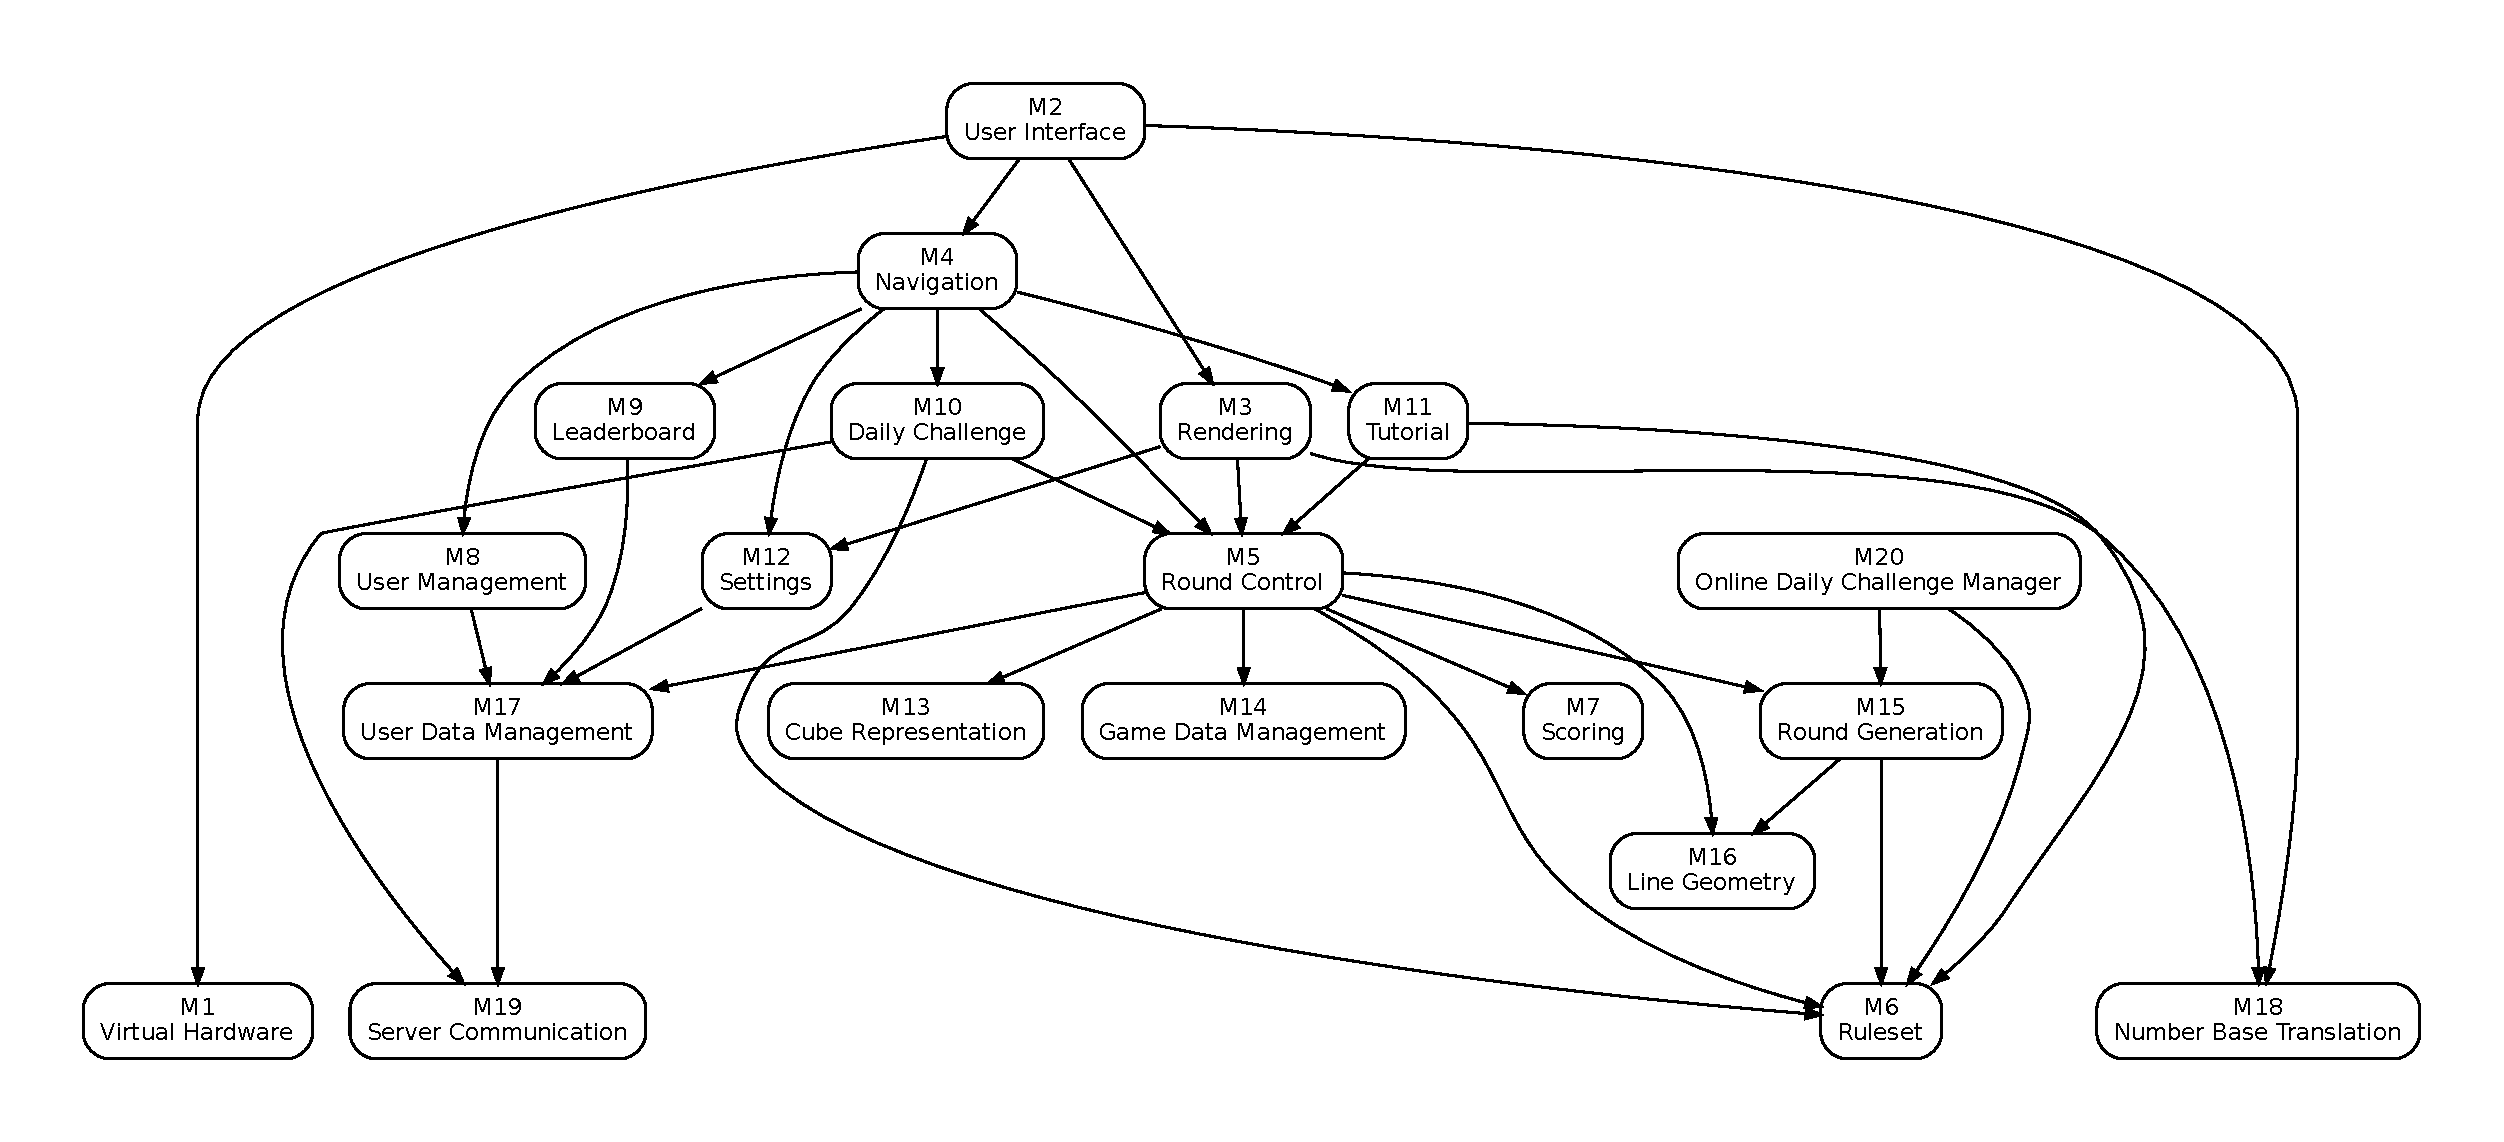
\includegraphics[width=\textwidth]{UsesHierarchy.pdf}
\caption{Use hierarchy among modules}
\label{FigUH}
\end{figure}

%\section*{References}

\section{User Interfaces}

\wss{Design of user interface for software and hardware.  Attach an appendix if
needed. Drawings, Sketches, Figma}

\section{Design of Communication Protocols}

\wss{If there is communication between hardware and software, it may be necessary 
to explain the design of the communication protocol.  This section should be filled 
in with NA if it is not appropriate for a given project.}

\section{Database Design}

\wss{If a database is a significant component of the project, the database
design should be summarized here.  This section should be filled in with NA if
it is not appropriate for a given project.}

\section{Timeline}

\wss{Schedule of tasks and who is responsible}

\wss{You can point to GitHub if this information is included there}

\section{Generative AI Use Disclosure}

\wss{ChatGPT (version 5) was used to brainstorm ideas for the template for this disclose section.}

\subsection{AI Tools Used}

\wss{Give the name of the AI tool(s) used and the version.}

Microsoft Copilot version 155.0 and Claude Opus version 5.5 were used in support of completing this document.

\subsection{How and Where Used}

\wss{Explain what the tool(s) were used for.  Examples include: brainstorming,
explaining a technical concept, reviewing the document, generating or modifying
text, generating or modifying diagrams, identifying errors or omissions or
inconsistencies.}

\wss{For each of the uses, identify which parts of the document were affected.}

\wss{You do not need to report every interaction, but you should disclose the 
uses that materially contributed to your work}

Generative AI was useful in reading the assignment description, previous work, and our iterations of the document to provide recommendations (especially related to consistency with SRS). For example, after writing the initial version of the ACs, UCs, and modules as well as the ideas for the secrets, Generative AI was used to identify potential ambiguities or suggest additional content (e.g., suggesting new modules and ACs that aligned with the SRS requirements). Generative AI was also useful in helping to plan how the modules interacted with each other and in particular, how they use each other (for the Use Hierarchy); Generative AI was used to suggest potential design options which we then went through and refined until we had a design we liked. Generative AI was also used to create the Uses Hierarchy .dot file. Additionally, Generative AI was used to create the traceability table between ACs and Modules. Finally, Generative AI was useful in drafting some important clarification paragraphs such as the AC to SRS LC explanation and the additional explanation for the Uses Hierarchy.

\subsection{Verification of AI-Generated Content}

\wss{\begin{itemize}
    \item Describe how the team checked AI-generated or AI-assisted material
    before including it in the document.
    \item In particular, verify factual claims, technical assertions,
    requirements, calculations, references, and other information for which an
    AI system may produce incorrect or fabricated results.
    \item \textbf{The team is responsible for the accuracy, completeness,
consistency, and appropriateness of the submitted document, regardless of
whether material was generated by a human or an AI system.}
\end{itemize}}

The suggestions provided by Microsoft Copilot and Claude were not blindly implemented. Instead, to ensure the content was reasonable/quality and fit the tone and intent of our document, the suggestions/revisions were reviewed by a team member and then edited as required before being added. References to requirements or other documents were manually reviewed to ensure they made sense and were accurate.

\newpage{}

\bibliographystyle {plainnat}
\bibliography{../../../refs/References}

\end{document}